\documentclass[10pt,letterpaper]{article}
\usepackage[margin=0.7in,headheight=14pt]{geometry}
\usepackage[T1]{fontenc}
\usepackage{lmodern,amsmath,amssymb,booktabs,graphicx,xcolor,array}
\usepackage[colorlinks=true,urlcolor=blue,linkcolor=blue]{hyperref}
\hypersetup{pdftitle={Homework 3 Solutions},pdfauthor={Ruochen Wang}}
\pagestyle{myheadings}
\markright{\small Ruochen Wang \quad | \quad Foundations of Machine Learning and AI \quad | \quad HW3}
\setlength{\parindent}{0pt}
\setlength{\parskip}{5pt}
\setlength{\tabcolsep}{5pt}
\newcommand{\E}{\mathbb E}
\newcommand{\R}{\mathbb R}
\newcommand{\RFChoice}{RF selects 200 trees, unrestricted depth, minimum leaf size 1, feature fraction 0.33, and bootstrap fraction 1.0.}
\newcommand{\KNNChoice}{6 neighbors, inverse-distance weights, and Manhattan distance}
\newcommand{\WineRows}{Random forest & 0.0506 & 0.3051 & 0.4301 & +0.1250 \\
K-nearest neighbors & 0.0000 & 0.3359 & 0.4778 & +0.1419 \\
Training-mean baseline & 0.7839 & 0.7417 & 0.8067 & +0.0650 \\}
\newcommand{\WineInterpretation}{RF's test MSE is 0.1250 higher than its selected validation MSE; KNN's test MSE is 0.1419 higher than its selected validation MSE. Validation and test estimate the risk of the same fitted predictor, but on different samples. Validation also influenced which predictor was selected. Their difference reflects both selection and sampling variability; its sign on one split is not a proof or disproof of the expected optimism in part (b). Both selected models improve on the constant baseline on the test set.}
\newcommand{\WineDuplicates}{937}
\newcommand{\WineValRepeats}{114}
\newcommand{\WineTestRepeats}{253}
\newcommand{\BoostRows}{dset0 & 1 & 42.57 & 42.67 & 0.65915 & 0.6785 \\
dset0 & 10 & 15.14 & 27.33 & 0.50015 & 0.5770 \\
dset0 & 100 & 0.29 & 15.33 & 0.12270 & 0.4144 \\
dset0 & 300 & 0.00 & 13.33 & 0.01861 & 0.4969 \\
dset0 & 1,000 & 0.00 & 17.33 & 0.00007 & 1.0119 \\
\midrule
dset1 & 1 & 24.00 & 24.67 & 0.63682 & 0.6459 \\
dset1 & 10 & 12.57 & 18.67 & 0.40185 & 0.4825 \\
dset1 & 100 & 1.14 & 14.67 & 0.11775 & 0.3210 \\
dset1 & 300 & 0.00 & 15.33 & 0.02169 & 0.3944 \\
dset1 & 1,000 & 0.00 & 16.67 & 0.00012 & 0.7376 \\}
\newcommand{\SensitivityRows}{dset0 & $17.93\pm2.85$ & $17.63\pm2.90$ & $17.90\pm2.80$ \\
dset1 & $18.63\pm2.98$ & $19.53\pm2.86$ & $19.93\pm2.84$ \\}

\begin{document}
\begin{center}
{\LARGE\bfseries Homework 3 Solutions}\\[6pt]
{\large Ruochen Wang}\\[3pt]
Data 37711: Machine Learning \& AI Part I \quad Fall 2026
\end{center}
\textbf{Course repository:} \url{https://github.com/richard0525/foundations-machine-learning-ai}\\
\textbf{HW3 code, data, and results:} \href{https://github.com/richard0525/foundations-machine-learning-ai/tree/main/homework_3}{\texttt{homework\_3/}} \quad
\href{https://github.com/richard0525/foundations-machine-learning-ai/blob/main/homework_3/README.md}{Run instructions}

\section*{1. Poisson regression with boosting}
\textbf{(a)(i) Choice of distribution.}
A Poisson random variable takes values $0,1,2,\ldots$, making it a natural starting model for a nonnegative count. Write its conditional rate as $m(x)>0$:
\[
\Pr(Y=y\mid X=x)=\frac{e^{-m(x)}m(x)^y}{y!},\qquad
\E[Y\mid x]=\operatorname{Var}(Y\mid x)=m(x).
\]
Matching the support motivates this choice; the additional mean--variance equality is a modeling assumption, not a consequence of being count-valued.

\textbf{(a)(ii) Exponential transformation.}
The additive tree score $f(x)=\sum_j\lambda_jh_j(x)$ can be any real number. Setting $m(x)=e^{f(x)}$ guarantees a positive rate while allowing unrestricted real tree outputs. Thus $f(x)$ is the log-rate and $e^{f(x)}$ is the predicted mean count. In standard GLM terminology, $\log$ is the link and $\exp$ its inverse.

\textbf{(b) Loss.}
Substitute $m=e^f$ into the probability mass function and take its negative logarithm:
\begin{align*}
\log p(y\mid f)&=-e^f+y\log(e^f)-\log(y!)=-e^f+yf-\log(y!),\\
L(y,f)&=\boxed{e^f-yf+\log(y!)},\qquad
\widehat R(f)=\frac1n\sum_{i=1}^n L(y_i,f(x_i)).
\end{align*}
The $\log(y!)$ term does not depend on the model, so it may be dropped during optimization. The full expression is the Poisson negative log-likelihood.

\textbf{(c) Derivative with respect to the score.}
\[
\boxed{\frac{\partial L(y,f)}{\partial f}=e^f-y},\qquad
\frac{\partial^2L(y,f)}{\partial f^2}=e^f>0.
\]

\textbf{(d) First-order boosting.}
Initialize with the best constant score $f_0=\log\bar y$ when $\bar y>0$. For each round $t$:
\begin{align*}
 r_{it}&=-\left.\frac{\partial L(y_i,f)}{\partial f}\right|_{f=f_{t-1}(x_i)}
       =y_i-e^{f_{t-1}(x_i)},\\
 h_t&\approx\underset{h\in\mathcal H_{\rm tree}}{\arg\min}
          \sum_{i=1}^n\big(r_{it}-h(x_i)\big)^2,\\
 f_t(x)&=f_{t-1}(x)+\eta_t h_t(x).
\end{align*}
Fit a regression tree to the negative-gradient targets, and use a small positive step $\eta_t$ or a line search on the original training Poisson loss. The assignment's $\lambda_t$ absorbs this step. At prediction time, return $\widehat m(x)=e^{f_T(x)}$. The tree's least-squares fit approximates a descent direction; the overall objective remains Poisson loss. If all observed counts are zero, the best constant rate is approached as $f_0\to-\infty$; a finite implementation can use a positive rate floor.

\newpage
\section*{2. Hyperparameter selection}
\textbf{(a) A finite-candidate generalization bound.}
Let $K$ denote the number of complete configurations tried. Thus $K=k$ if $k$ counts configurations; if $k$ counts parameter axes with $m_a$ choices each, use $K=\prod_{a=1}^k m_a$ instead.

Condition on the training set of size $n$ and the training random seeds, denoted $T$. The fitted candidates $f_1,\ldots,f_K$ are then fixed. Assume the evaluation set $Z_1,\ldots,Z_l$ is i.i.d. and independent of $T$, that the candidate list is specified without its outcomes, and that $0\le L(Y,f_j(X))\le B$ almost surely for every $j$. Define
\[
R_j=\E[L(Y,f_j(X))\mid T],\qquad
\widehat R_j=\frac1l\sum_{i=1}^l L(Y_i,f_j(X_i)),\qquad
\hat j\in\arg\min_j\widehat R_j.
\]
For any fixed candidate, two-sided Hoeffding gives
\[
\Pr\big(|\widehat R_j-R_j|>\epsilon\mid T\big)
\le 2\exp\!\left(-\frac{2l\epsilon^2}{B^2}\right).
\]
Taking a union bound over all $K$ candidates,
\[
\Pr\!\left(\max_{1\le j\le K}|\widehat R_j-R_j|>\epsilon\mid T\right)
\le 2K\exp\!\left(-\frac{2l\epsilon^2}{B^2}\right).
\]
For $0<\delta<1$, set the right-hand side to $\delta$ and solve for $\epsilon$. With probability at least $1-\delta$,
\[
\boxed{\;|\widehat R_{\hat j}-R_{\hat j}|\le
B\sqrt{\frac{\log(2K/\delta)}{2l}}\;}.
\]
This holds for the selected model because the event protects all candidates simultaneously. Integrating over $T$ gives the same unconditional guarantee. The candidates need not be independent of one another. The evaluation size $l$ controls this estimation gap; $n$ affects the fitted models but does not appear in this conditional bound. It is nonvacuous relative to the largest possible gap $B$ when $\log(2K/\delta)<2l$.

The bounded-loss assumption matters: arbitrary unbounded squared loss has no such distribution-free guarantee from $n,l,K$ alone. For example, with predictor zero, let $Y=\sqrt M$ with probability $p$ and zero otherwise. The true MSE is $pM$, but the evaluation MSE is zero with probability $(1-p)^l$; $M$ can be arbitrarily large. In part (c), assuming the stated target range $[1,10]$, RF and KNN predictions stay within the training-label range, so $B=81$ is valid.

\textbf{(b) Reusing the selection set.}
Choosing the smallest evaluation loss selects partly for favorable sampling noise. In fact, conditional on the fixed fitted candidates,
\[
\E[\widehat R_{\hat j}\mid T]
=\E[\min_j\widehat R_j\mid T]
\le\min_j R_j
\le\E[R_{\hat j}\mid T].
\]
The reported selection score is therefore optimistic \emph{in expectation}. A larger $K$ or smaller $l$ increases the opportunity for selection overfitting, reflected by the $\sqrt{\log K/l}$ allowance. There is no sharp failure threshold at $K=l$, and a particular test loss can still be below the selected validation loss.

The set used to choose hyperparameters functions as a \emph{validation} set, even if called ``test.'' Use training data to fit, validation data to choose the configuration, and a separate untouched test set to estimate the selected model's performance. Models newly invented after inspecting validation outcomes require more than a union bound over an otherwise unfixed list.

\newpage
\section*{2(c). White-wine regression experiment}
\textbf{Data and protocol.}
I used the white-wine CSV from the linked UCI Wine Quality archive [1]: 4,898 observations, 11 physicochemical predictors, and the last column, \texttt{quality}, as the response. The supplied folder contained the two part-3 datasets; the wine file was downloaded from UCI. The observed quality range is 3--9. Random row splits give 3,428 training, 490 validation, and 980 test observations. First reserve 20\% using seed 2026; split the remaining rows with validation fraction $1/8$ and seed 2027.

KNN inputs are standardized using training means and standard deviations only. RF uses the original inputs. Every candidate is fitted on training data and ranked by validation MSE, $N^{-1}\sum_i(y_i-\hat y_i)^2$. Exact ties use the first configuration in a fixed grid order. Both selections are frozen before test evaluation; the selected models remain fitted on training data only.

\textbf{Search spaces.} Parameter meanings follow the scikit-learn documentation [2,3].
\begin{center}\small
\begin{tabular}{@{}llp{2.65in}@{}}
\toprule Model & Parameter & Values and role \\ \midrule
RF & \texttt{n\_estimators} & $50,100,200$: number of averaged trees.\\
& \texttt{max\_depth} & None, $3,5,10,20$: maximum tree depth.\\
& \texttt{min\_samples\_leaf} & $1,2,4,8$: minimum observations in a leaf.\\
& \texttt{max\_features} & $0.33,0.66,1.0$: feature fraction considered per split.\\
& \texttt{max\_samples} & $0.6,0.8,1.0$: bootstrap sample size as a fraction of training rows.\\ \midrule
KNN & \texttt{n\_neighbors} & Every integer $1,\ldots,125$: neighborhood size.\\
& \texttt{weights} & Uniform or inverse-distance weighting.\\
& \texttt{p} & $1$ (Manhattan) or $2$ (Euclidean) distance.\\ \bottomrule
\end{tabular}
\end{center}
RF uses bootstrap sampling, squared-error splits, and random seed 2026; KNN uses exact brute-force neighbor search. The RF grid has $3\cdot5\cdot4\cdot3\cdot3=540>490$ configurations; the KNN grid has $125\cdot2\cdot2=500>490$.

\textbf{Selected configurations.} \RFChoice\ KNN selects \KNNChoice.

\textbf{Results.} The baseline predicts the training-set mean. KNN training error includes each row as its own zero-distance neighbor; it is not leave-one-out error.
\begin{center}
\begin{tabular}{@{}lrrrr@{}}
\toprule Model & Train MSE & Validation MSE & Test MSE & Test $-$ val. \\\midrule
\WineRows
\bottomrule
\end{tabular}
\end{center}
\WineInterpretation

\textbf{Scope of the split.} The wine data contain \WineDuplicates\ exact duplicate rows beyond their first occurrences. Under the assignment's random-row split, \WineValRepeats\ validation rows and \WineTestRepeats\ test rows exactly match a training record (all features and quality). These rows are retained. The test scores describe this row-sampling protocol; they need not describe performance on wholly distinct wines. The saved split indices, all 1,040 candidate scores, and predictions are in \texttt{results/}.

\newpage
\section*{3. Boosting and the number of trees}
\textbf{Shared protocol.}
The supplied \texttt{dset0-1.csv} and \texttt{dset1-1.csv} correspond to dset0 and dset1. Each is read \emph{without a header}: 500 observations, a binary target in the first column, and five predictors. Each dataset is split into 350 training and 150 test observations by stratified random sampling with seed 2026.

I fit \texttt{GradientBoostingClassifier} [4] with binary log loss, learning rate $0.1$, maximum depth 3, full-sample boosting, model seed 2026, and no early stopping. All other settings are fixed across tree counts. The requested five budgets are evaluated without selecting a model on test data. Independent fits at those budgets agree exactly with the corresponding prefixes of the 1,000-tree fit. Error uses the predicted class; log loss is computed stably from the real score $f$ as $\log(1+e^f)-yf$.

\textbf{(a) dset0 and (b) dset1: measured performance.}
\begin{center}\small
\begin{tabular}{@{}llrrrr@{}}
\toprule Data & Trees & Train error (\%) & Test error (\%) & Train log loss & Test log loss\\\midrule
\BoostRows
\bottomrule
\end{tabular}
\end{center}
\begin{center}
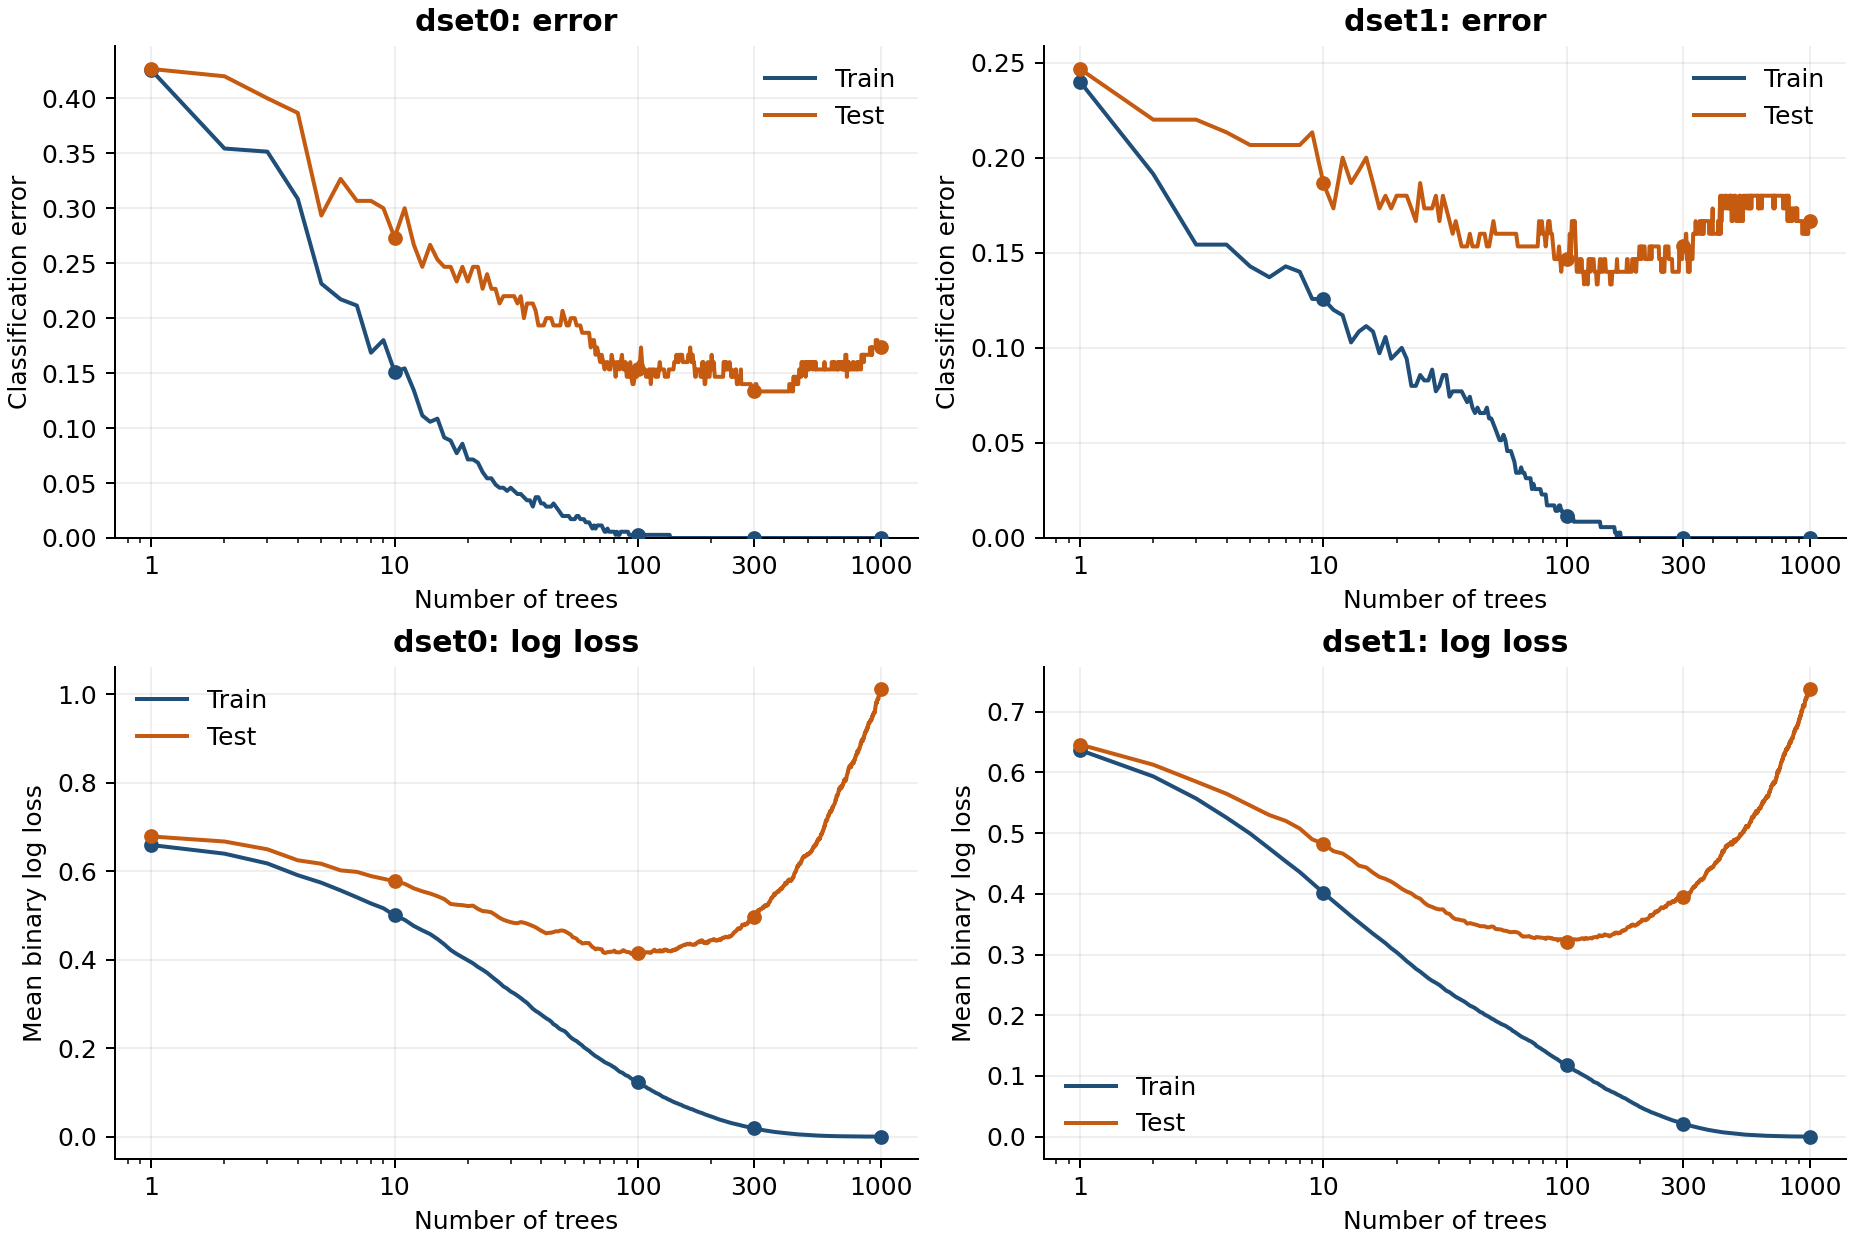
\includegraphics[width=.98\linewidth]{results/figures/q3_learning_curves.png}
\end{center}
\vspace{-5pt}
{\small\textbf{Figure 1.} Training and held-out performance along the fixed boosting paths. Dots mark the five required tree counts; the horizontal axis is logarithmic.}

\newpage
\section*{3. Interpretation and comparison}
\textbf{(a) dset0.}
Test classification error falls from 42.67\% at one tree to 13.33\% at 300 trees, then rises to 17.33\% at 1,000. Training error reaches zero by 300 trees and stays there. Among the five requested budgets, test log loss is smallest at 100 trees (0.4144) and rises to 1.0119 at 1,000. Thus improving the training objective eventually harms held-out performance; the 0--1 error and probability-sensitive log loss need not favor the same budget.

\textbf{(b) dset1.}
Test error improves from 24.67\% at one tree to 14.67\% at 100, then increases to 16.67\% at 1,000. Training error again reaches zero by 300. Test log loss falls to 0.3210 at 100 trees and then rises to 0.7376. Additional rounds can make the remaining wrong predictions more confident even while training loss keeps falling. These observed minima describe the experiment; they are not a test-selected deployment recommendation.

\textbf{(c) What could explain the differences?}
dset1 has a stronger simple marginal signal: the sample correlation between the label and the first predictor is $-0.589$, versus $0.032$ in dset0. This is consistent with its faster early improvement. In dset0, the first feature nonetheless receives substantial fitted tree importance, suggesting that marginal correlation misses nonlinear or interaction structure. These are descriptive clues, not identification of the data-generating mechanism.

Both datasets exhibit late overfitting in log loss. Overlapping classes, noisy labels, difficult boundary points, or irrelevant inputs can cause later trees to fit sample-specific patterns and become overconfident. The observed samples are not strictly linearly separable (checked by linear-program feasibility), but that does not prove label noise: a clean nonlinear boundary could also explain this. Zero training error from flexible trees likewise does not establish a noise-free population.

\textbf{Sensitivity to the random split.}
Repeating the same fixed experiment for 20 prespecified stratified split seeds $0,\ldots,19$, with the model seed still 2026, gives:
\begin{center}\small
\begin{tabular}{@{}lrrr@{}}
\toprule & \multicolumn{3}{c}{Mean test error $\pm$ SD (percentage points)}\\
Data & 100 trees & 300 trees & 1,000 trees\\\midrule
\SensitivityRows
\bottomrule
\end{tabular}
\end{center}
The late classification error is nearly flat for dset0 and increases modestly for dset1. Mean test log loss from 100 to 1,000 trees rises from 0.4197 to 0.9179 for dset0 and from 0.4079 to 1.0739 for dset1. The splits overlap, so the reported SD describes split sensitivity, not a confidence interval. These results support a cautious comparison rather than a claim that one dataset never overfits.

\vspace{3pt}
\textbf{References and files.}\\[-2pt]
{\small
[1] P. Cortez et al. (2009), \emph{Wine Quality}, \href{https://archive.ics.uci.edu/dataset/186/wine+quality}{UCI dataset}; \href{https://archive.ics.uci.edu/static/public/186/wine+quality.zip}{source archive}.\par
[2] scikit-learn 1.7.2, \href{https://scikit-learn.org/1.7/modules/generated/sklearn.ensemble.RandomForestRegressor.html}{RandomForestRegressor documentation}.\par
[3] scikit-learn 1.7.2, \href{https://scikit-learn.org/1.7/modules/generated/sklearn.neighbors.KNeighborsRegressor.html}{KNeighborsRegressor documentation}.\par
[4] scikit-learn 1.7.2, \href{https://scikit-learn.org/1.7/modules/generated/sklearn.ensemble.GradientBoostingClassifier.html}{GradientBoostingClassifier documentation}.\par
Full experiment commands and pinned dependencies: \href{https://github.com/richard0525/foundations-machine-learning-ai/blob/main/homework_3/README.md}{\texttt{homework\_3/README.md}}. Numerical results, plots, and predictions: \href{https://github.com/richard0525/foundations-machine-learning-ai/tree/main/homework_3/results}{\texttt{homework\_3/results/}}.
}
\end{document}
